XPath is a language for addressing parts of an XML document and is also used with other SGML bases standards as HTML. It is used to extract certains parts of an XML or HTML document in a easy way. In support of this primary purpose, it also provides basic facilities for manipulation of strings, numbers and booleans.\\

XPath operates on the abstract, logical structure of a document, rathyer than its surface syntax. If the developer can describe what data is searching for using the XPath language, the parser can fetch it or point the program to the right path in the document, usually with just a single line.\\

\section{Basic Concepts}

\subsection{Tree}

XPath models a document as a tree of nodes. There are different types of nodes like element nodes, attribute nodes and text nodes.\\

The primary syntactic construct in XPath is the expression. An expression matches the production Expr. An expression is evaluated to yield an object, which has one of the following four basic types:\\

\begin{itemize}
	\item nodeset
	\item boolean
	\item number
	\item string
\end{itemize}

For example if we have this XML document:

\newpage

\lstset{language=XML, caption=XML document, frame=shadowbox, rulesepcolor=\color{blue}, inputencoding=utf8x}

\begin{lstlisting}
<?xml version="1.0" encoding="UTF-8"?>

<network>
    <description name="Boston">
        This is the configuration of our network in the Boston office.
    </description>
    <host name="agatha" type="server" os="linux">
        <interface name="eth0" type="Ethernet">
            <arec>agatha.example.edu</arec>

            <cname>mail.example.edu</cname>
            <addr>192.168.0.4</addr>
        </interface>
        <service>SMTP</service>

        <service>POP3</service>
        <service>IMAP4</service>
    </host>
    <host name="gil" type="server" os="linux">
        <interface name="eth0" type="Ethernet">

            <arec>gil.example.edu</arec>
            <cname>www.example.edu</cname>
            <addr>192.168.0.5</addr>
        </interface>

        <service>HTTP</service>
        <service>HTTPS</service>
    </host>
    <host name="baron" type="server" os="linux">
        <interface name="eth0" type="Ethernet">

            <arec>baron.example.edu</arec>
            <cname>dns.example.edu</cname>
            <cname>ntp.example.edu</cname>
            <cname>ldap.example.edu</cname>

            <addr>192.168.0.6</addr>
        </interface>
        <service>DNS</service>
        <service>NTP</service>

        <service>LDAP</service>
        <service>LDAPS</service>
    </host>
    <host name="mr-tock" type="server" os="openbsd">
        <interface name="fxp0" type="Ethernet">

            <arec>mr-tock.example.edu</arec>
            <cname>fw.example.edu</cname>
            <addr>192.168.0.1</addr>
        </interface>

        <service>firewall</service>
    </host>
    <host name="krosp" type="client" os="osx">
        <interface name="en0" type="Ethernet">
            <arec>krosp.example.edu</arec>

            <addr>192.168.0.100</addr>
        </interface>
        <interface name="en1" type="AirPort">
            <arec>krosp.wireless.example.edu</arec>
            <addr>192.168.100.100</addr>

        </interface>
    </host>
    <host name="zeetha" type="client" os="osx">
        <interface name="en0" type="Ethernet">
            <arec>zeetha.example.edu</arec>

            <addr>192.168.0.101</addr>
        </interface>
        <interface name="en1" type="AirPort">
            <arec>zeetha.wireless.example.edu</arec>
            <addr>192.168.100.101</addr>

        </interface>
    </host>
</network>
 \end{lstlisting}


The tree parsed by XPath will be like Figure \ref{graf:xml-tree}.\\

The root of the tree points to $<network></network>$  and the other elements of the document hang off the root. Each element node has attribute nodes (if it has any attributes)and a child text node that represents the contents of that element (if it has any character data in it). \cite{Blank-Edelm} \\

\begin{figure}[ht!]
   \centering
   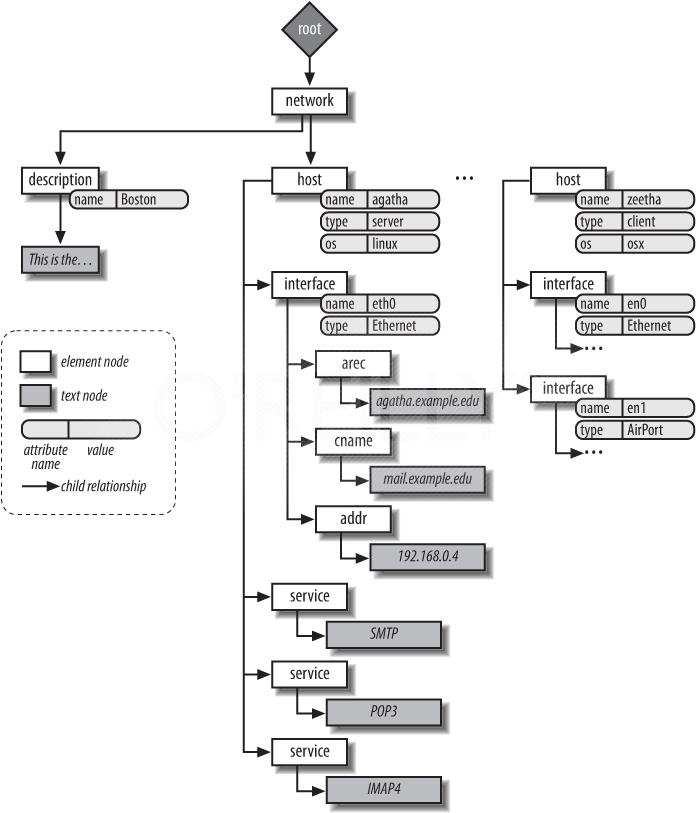
\includegraphics[scale=0.6]{imgs/xml-tree.png}
   \caption{XML tree}\label{graf:xml-tree}
\end{figure}

\newpage

\subsection{Location}

\subsubsection{Absolute Path}


If this diagram reminds you of a file system, that’s good. The resemblance is intentional. XPath uses the concept of a location path to navigate to a node or set of nodes in a document. Location paths start either at the top of the tree (an absolute path) or at some other place in the tree (a relative path). Just like in a filesystem, “/” at the beginning means “start at the root of the tree,” “.” (dot) refers to the current node (also known as the “context node”), and “..” (dot-dot) refers to the parent of the context node. \cite{Blank-Edelm} \\

As explained. to start at the root of the system we use "/", for example if we wanted to point at the $<description> </description>$ node the location path would be /network/description and we will obtain the description node.\\


\begin{lstlisting}[frame=none, title=Nodes]
<description></description>
\end{lstlisting} 


\subsubsection{Relative Path}

We also can use the relative path to point at a node or nodeset using "//", for example if we want to obtain all the host nodes, the location path will be //host and the result will be all the host nodes:\\

\begin{lstlisting}[frame=none, title=host nodes]
<host name="agatha"></host>
<host name="gil"></host>
<host name="baron"></host>
<host name="mr-tock"></host>
<host name="krosp"></host>
<host name="zeetha"></host>
\end{lstlisting}

You can also place double slashes in the middle of a location path, as in \textbf{/network//service/text()}. The sample file has a very simple node tree, but you can imagine how the ability to describe a path without specifying all of the intervening parts of the tree can be usefull.\\

Wildcards in XPath can function similarly to their filesystem analogs. \textbf{/network/host/*/arec/text()} finds all element nodes under a $<host></host>$ node that have $<arec> </arec>$ sub-nodes and then returns the contents of those $<arec></arec>$ elements. In this case, we get back the DNS A resource record name associated with each interface:\\

\begin{itemize}
\item agatha.example.edu
\item gil.example.edu
\item baron.example.edu
\item mr-tock.example.edu
\item krosp.example.edu
\item krosp.wireless.example.edu
\item zeetha.example.edu
\item zeetha.wireless.example.edu
\end{itemize}

Attributes can be wildcarded in a similar fashion by using @*. /network/host/@* would return all of the attributes of the <host></host> elements.\\

\subsection{Attributes}

Many nodes have attributes and/or text labels. To get an element's attribute, we use @ in fornt of the attribute name. For example, \textbf{/network/description/@name} gets us name="Boston". To access the contents of an element’s text node, we end the location path with text(), as in \textbf{/network/description/text()}. This returns the data \textit{This is the configuration...}.\\

We can also select a node's children using relative location paths. For example we can use the path:\\

\textbf{/description/*}\\

And obtain the text children of description.\\

\subsection{Predicates}

In our example document, we have five $<host></host>$ elements at the third level of the tree. They have different attributes and the data in each is different, but that doesn’t help if the location path is constructed with just element names. If we say \textbf{/network/host}, all the hosts are selected, the path is not giving us the granularity needed to select a single node.\\

For this granularity is that Predicates are used. They allow us to filter the set of possible to get just the ones needed. Predicates are specified in square brackets ([]) in the location path itself. You insert a predicate right at the point where a filtering decision has to be made.\\

The simplest predicate example looks like an index number, as in \textbf{/network/host[2]/interface/arec/text()}. This location path returns the interface name(s) for the second host node (second in document order). If you were standing and looking at all of the host nodes, the predicate would tell you which branch of the tree to take: in this case, the one in the second position.\\

Index number are not the only possible predicates. XPath has a relatively rich set of predicates available for use. The next level of predicate complexity looks something like this: \textbf{/network/host[@name="agatha"]}. This selects the correct $<host></host>$ by testing for the presence of a specific attribute with a specific value.\\

If we want to find the name of all the Linux servers in the network, we could write the location path \textbf{/network/host[@os="linux"]/service/../@name}. Here we use a predicate to select all the $<host></host>$ that have an \textbf{os} attribute of \textbf{linux}. Then it search down the branch for each $<service></service>$ node (in fact selecting all the hosts that are servers). With ../@name we get tha name attribute of its parent, the $<host></host>$ that contains the $<service></service>$ we just found. \cite{Blank-Edelm}\\

We can test the contents of a node like this: \textbf{//host/service[text()='DNS']}. This location path says to start at the root of the tree looking for branches that have a $<service></service>$ node embedded in a $<host></host>$ node. Once XPath finds a branch that fits this description, it compares the contents of each of those service nodes to find the one whose contents are “DNS”.\\

If we want only the HTTP and HTTPS service nodes we can use \textbf{//host/service[starts-with(normalize-space(.),'HTTP')]}.\\

For a list of available predicates you can read:\\

\url{http://www.w3.org/TR/xpath/#predicates}\\


\section{Unabbreviated Syntax}

Until now we have been using the \textit{abbreviated syntyax}, and you will use it in most of the cases, but sometimes is good to know the \textit{Unabbreviated Syntax} for some difficult cases.\\

If we use the location path \textbf{/network/host[2]/service[1]/text()} what are we doing is:\\

\begin{enumerate}
\item Start at the root of the tree.
\item Go down the tree), looking for the child node or nodes with the element name \textbf{network}.
\item Arrive at the $<network></network>$ node. This becomes the context node.
\item Walk toward the children of the context node, looking for the child node or nodes with the element name \textbf{host}.
\item Arrive at the level in the tree that has several $<host></host>$ nodes. Filter to choose the node in the second position. This becomes the context node.
\item Walk toward the children of the context node, looking for the child node or nodes with the element name \textbf{service}.
\item Arrive at the level in the tree that has several $<service></service>$ nodes. Filter to choose the node in the first position. This becomes the context node.
\item Walk toward the \textbf{text node} associated with the context node. End.
\end{enumerate}

In the unabbreviated syntax it woul look like the following:\\

\textbf{/child::network/child::host[position()=2]/child::service[position()=1]/child::text()}\\

What we had add to the location path ere the axes, each axis tell the parser in which direction to move in the tree relative to the context node. In this case each step is moving in the \textit{child} direction. XPath doesn’t restrict us to moving from child node to child node down the tree. We’ve seen one example of this freedom already with the // syntax. When we say \textbf{/network//cname}, we are really indicating \textbf{/child::network/descendant-or-self::cname}. That is:\\

\begin{enumerate}
\item Start from the root.
\item Move to its child nodes to find a $<network></network>$ node or nodes. When we find one, it becomes the context node.
\item Look at the context node or descend farther in the tree until we find a $<cname></cname>$ node or nodes.
\end{enumerate}

The other three axes you already know how to reference in abbreviated form are \textbf{self:: (.)}, \textbf{parent:: (..)}, and \textbf{attribute:: (@)}. The unabbreviated syntax lets us use all of the other axes—eight more, believe it or not: \textbf{ancestor::}, \textbf{following-sibling::}, \textbf{preceding-sibling::}, \textbf{following::, preceding::}, \textbf{namespace::}, \textbf{descendant::}, and \textbf{ancestor-or-self::}.\\

The \textbf{following-sibling::} axis tells the parser to move over to the next element(s) in the tree at that level. This references the context node’s siblings. If we wanted to write a location path that tried to find all of the hosts with multiple interfaces, we could write:\\

\textbf{/child::network/child::host/child::interface/following-sibling::interface/}\\
\textbf{parent::host/attribute::name}\\

This says, “Walk down from the network node until you find a host with an interface node as its child, then see if it has a sibling interface at the same level in the tree. If it does, walk back up to the host node and return its name attribute.”\\

You can read more about the axes in:\\

\url{http://www.w3.org/TR/xpath/#axes}\\




